\chapter{Next steps}

%\textcolor{blue}{The scope of our project is relatively large. Because of this, we decided to divide the development into two main phases. The first we called the offline phase. The main goal during this step is to develop a model capable of signalling anomalous traffic in existing data sets. Using existing data sets will jump-start our development and allow quick iterations over different possibilities we want to explore. The second one is called the online phase. The main objective will be to test and validate the model found previously in a physical environment,i.e., connected to an existing vehicle ECU cluster. The detailed steps for both phases are listed below.}\par

Project development is split in two main phases: offline and online. The main goal of the offline phase is to develop a model capable of signalling anomalous traffic in existing data sets. Using these data sets will jump-start our development and allow quick iterations over different possibilities we want to explore. For the online phase, the main objective is to test and validate the model in a real environment, \textit{i.e.}, connected to an existing vehicle ECU cluster. The detailed steps for both phases are listed below.\par

The offline phase can be split into the following steps:
\begin{itemize}
    \item \textbf{Data set gathering}, where existing CAN data sets containing attacks are inspected and saved.
    \item \textbf{Exploration of possible models}, in which various machine learning approaches are investigated and attempted.
    \item \textbf{Analysis and choice of a model}, where a choice is made on the machine learning best approach to the problem.
    \item \textbf{Development of the IDS prototype}, where the proposed solution is implemented in code.
\end{itemize}

And the online phase is composed of these tasks:
\begin{itemize}
    \item \textbf{Definition of the test attacks}, in which various CAN attack procedures are investigated and a choice is made as to what will be attempted. 
    \item \textbf{Gathering of live data}, where data from a real vehicle cluster is gathered while attempting the chosen attacks.
    \item \textbf{Real-time testing of the model}, where the developed IDS is used to detect the attacks.
\end{itemize}

%\textcolor{blue}{We plan to write the final document in parallel with the development phase. This approach will ensure we do not forget any important details and findings. At the end of the project, there is still some buffer time reserved to conclude and improve the document.}\par

The writing of the final document is to be done in parallel with the development phase. This approach will ensure we do not forget any important details and findings. At the end of the project, there is still some buffer time reserved to conclude and improve the document. Figure \ref{fig:timeline} shows a Gantt chart with detailing the proposed timeline. Steps in blue are part of the offline phase of development, while the steps in green are part of the online phase. Orange signals the project's wrapping.

%\begin{itemize}
%    % ----- OFFLINE -----
%    \item Recolha de datasets                        - 7/02
%    \item Exploração dos vários modelos possíveis    - 31/03
%    \item Análise e escolha de o melhor modelo       - 15/05
%    % ----- ONLINE -----
%    \item Definição dos ataques de teste             - 31/05
%    \item Recolha de dados "reais"                   - 15/06
%    \item Teste do modelo em real time               - 15/07
%    
%    \item Finalizar documento                        - 31/07
%\end{itemize}

\begin{figure}
    \centering
    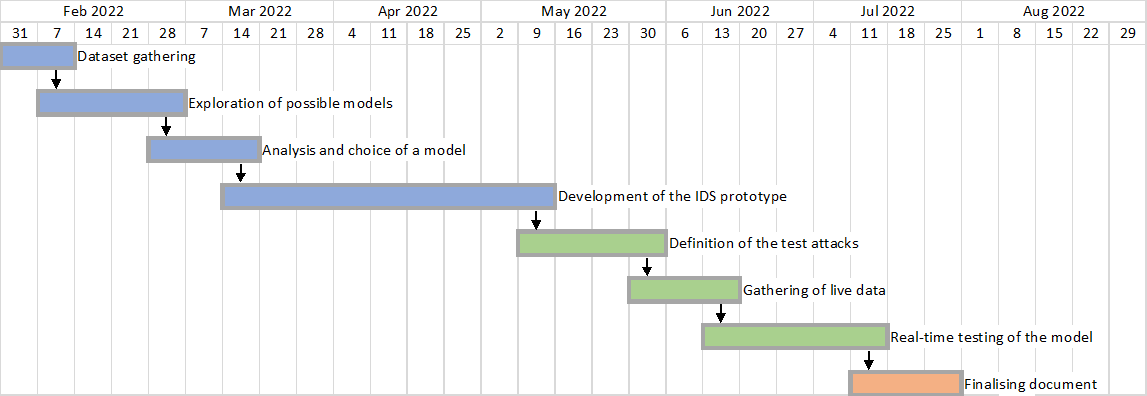
\includegraphics[width = \textwidth]{img/parts/conclusion/timeline.png}
    \caption{Project timeline (blue for the offline phase, green for the online phase, and orange for conclusion)}
    \label{fig:timeline}
\end{figure}